\chapter{State-of-the-Art}
%\chapter{Theoretische Grundlagen}
\label{ch:soa}

% This chapter can be also called Literature Review

Check what others have done, which is relevant to your research question and to provide evidence for testing the hypotheses defined in \autoref{sec:rq}.

For coherence: note that chapter titles should be \textit{Camel Cased}, while everything else is \textit{Sentence cased}, including all kinds of section names.

\section{Previous works}
\label{sec:prevworks}
	
% For referring to sections or chapter you rpesented before:
As explained in \citeA{negreiros2024database}.
	
	
\section{Types of something}
\label{sec:typesome}

Do \citeA{kundu2008fluid} talk about Lagrangian and Eulerian concepts visualized in \autoref{fig:example}?

\begin{figure}[htp]
	\begin{center}
		\begin{minipage}{\textwidth}
			\centering
			\resizebox*{.9\textwidth}{!}{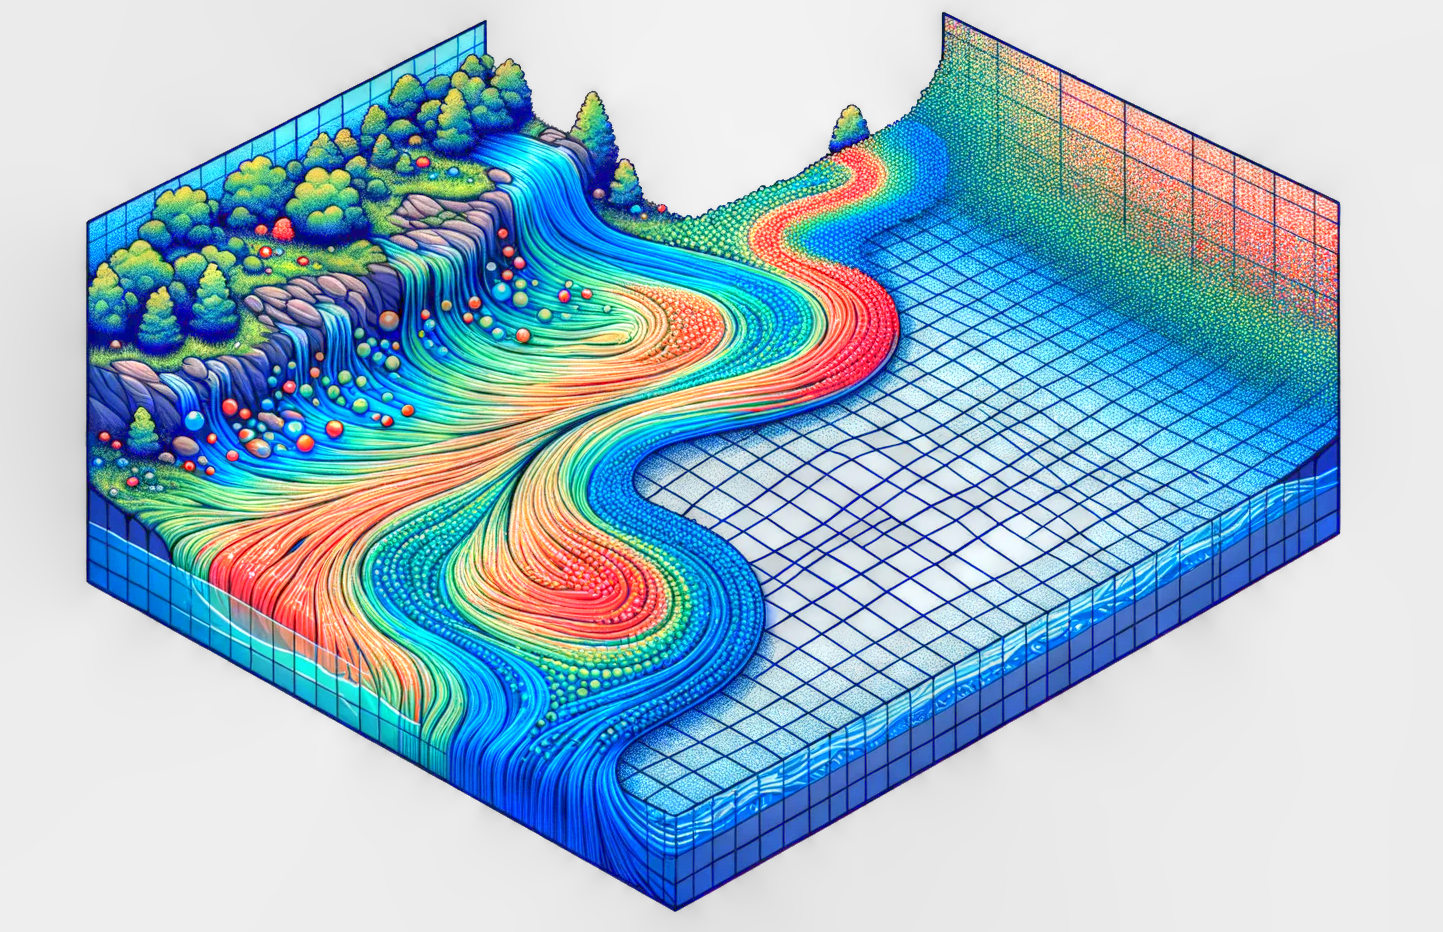
\includegraphics{example}}
			\caption[An example figure.]{An example figure that visually tries to integrate Lagrangian and Eulerian concepts.}
			\label{fig:example}
		\end{minipage}
	\end{center}
\end{figure}

		
\subsection{A subsection}
\label{subsec:somesome}
		
As the \autoref{tab:typesomething} shows, this text has to introduce the thing before the table lists the use of the thing.
		
		
\begin{table}[hb] % try [h]ere, then [b]ottom to make sure the table is mentioned in the text before it is shown
	\centering
	\caption{Captions of tables should be positioned above the table, while figure captions should be in the bottom}
	\begin{tabular}{ll}
		\hline
		\textbf{Thing} & \textbf{Use} \\
		\hline
		something & something \\
		something & something \\
		something & something \\
		\hline
	\end{tabular}
	% the label goes below the tabular env
	\label{tab:typesomething}
\end{table}
		
\subsection{No subsection goes alone}
\label{subsec:somenoth}

And it should also have some text.


\section{Something statistics}
\label{sec:somestatistics}
	
As shown in \autoref{eq:happiness}
\begin{equation}\label{eq:happiness}
	\mbox{happiness}=\frac{\mbox{EmptyCup}+\mbox{FavoriteDrink}}{\mbox{EmptyCups}}
\end{equation}	
	
\section{A section header}
\label{sec:some-ref}
	
\subsection{The logic underlying something}
\label{subsec:logicunderlying}
    	
\defbox{The thing}{
	This is the definition of the thing.
}
    	
\subsection{Concepts and terminology}
\label{subsec:conceptsterm}	
		
\subsubsection*{Something set rules} 

Understanding the semantics of something

\section{Something or nothing?}
\label{sec:someornot}

\subsubsection*{Unnumbered non-sense header?}

\infobox{The note}{
	Do you really need to do so much numbering?
}
   	
    	
    
